\documentclass[a5paper, 10pt]{article}

% Текст
\usepackage[utf8]{inputenc} % UTF-8 кодировка
\usepackage[russian]{babel} % Русский язык
\usepackage{indentfirst} % красная строка в первом параграфе в главе
% Отображение страниц
\usepackage{geometry} % размеры листа и отступов
\usepackage{listings}
\usepackage{color}

\geometry{
	left=12mm,
	top=25mm,
	right=15mm,
	bottom=17mm,
	marginparsep=0mm,
	marginparwidth=0mm,
	headheight=10mm,
	headsep=7mm,
	nofoot}
\usepackage{afterpage,fancyhdr} % настройка колонтитулов
\pagestyle{fancy}
\fancypagestyle{style}{ % создание нового стиля style
	\fancyhf{} % очистка колонтитулов
	\fancyhead[LO, RE]{Лабораторная работа № 7 } % название документа наверху
	\fancyhead[RO, LE]{Задачи 1650, 1450, 1806} % название section наверху
	\fancyfoot[RO, LE]{\thepage} % номер страницы справа внизу на нечетных и слева внизу на четных
	\renewcommand{\headrulewidth}{0.25pt} % толщина линии сверху
	\renewcommand{\footrulewidth}{0pt} % толцина линии снизу
}
\fancypagestyle{plain}{ % создание нового стиля plain -- полностью пустого
	\fancyhf{}
	\renewcommand{\headrulewidth}{0pt}
}
\fancypagestyle{title}{ % создание нового стиля title -- для титульной страницы
	\fancyhf{}
	\fancyhead[C]{{\footnotesize
			Министерство образования и науки Российской Федерации\\
			Федеральное государственное автономное образовательное учреждение высшего образования
	}}
	\fancyfoot[C]{{\large 
			Санкт-Петербург, 2024
	}}
	\renewcommand{\headrulewidth}{0pt}
}

% Математика
\usepackage{amsmath, amsfonts, amssymb, amsthm} % Набор пакетов для математических текстов
%\usepackage{dmvnbase} % мехматовский пакет latex-сокращений
\usepackage{cancel} % зачеркивание для сокращений
% Рисунки и фигуры
\usepackage[pdftex]{graphicx} % вставка рисунков
\usepackage{wrapfig, subcaption} % вставка фигур, обтекая текст
\usepackage{caption} % для настройки подписей
\captionsetup{figurewithin=none,labelsep=period, font={small,it}} % настройка подписей к рисункам
% Рисование
\usepackage{tikz} % рисование
\usepackage{circuitikz}
\usepackage{pgfplots} % графики
% Таблицы
\usepackage{multirow} % объединение строк
\usepackage{multicol} % объединение столбцов
% Остальное
\usepackage[unicode, pdftex]{hyperref} % гиперссылки
\usepackage{enumitem} % нормальное оформление списков
\setlist{itemsep=0.15cm,topsep=0.15cm,parsep=1pt} % настройки списков
% Теоремы, леммы, определения...
\theoremstyle{definition}
\newtheorem{Def}{Определение}
\newtheorem*{Axiom}{Аксиома}
\theoremstyle{plain}
\newtheorem{Th}{Теорема}
\newtheorem{Lem}{Лемма}
\newtheorem{Cor}{Следствие}
\newtheorem{Ex}{Пример}
\theoremstyle{remark}
\newtheorem*{Note}{Замечание}
\newtheorem*{Solution}{Решение}
\newtheorem*{Proof}{Доказательство}
% Свои команды
\newcommand{\comb}[1]{\left[\hspace{-4pt}\begin{array}{l}#1\end{array}\right.\hspace{-5pt} } % совокупность уравнений
% Титульный лист
\usepackage{csvsimple-l3}
\newcommand*{\titlePage}{
	\thispagestyle{title}
	\begingroup
	\begin{center}
		%		{\footnotesize
			%			Министерство образования и науки Российской Федерации\\
			%			Федеральное государственное автономное образовательное учреждение высшего образования
			%		}
		%		
		\vspace*{6ex}
		
		{\small
			САНКТ-ПЕТЕРБУРГСКИЙ НАЦИОНАЛЬНЫЙ ИССЛЕДОВАТЕЛЬСКИЙ УНИВЕРСИТЕТ ИТМО	
		}
		
		\vspace*{2ex}
		
		{\normalsize
			Факультет систем управления и робототехники
		}
		
		\vspace*{15ex}
		
		{\Large \bfseries 
			Лабораторная работа № 7
		}
\vspace*{2ex}
	{\Large \bfseries 
			
"Задачи 1650, 1450, 1806"
		}
\vspace*{2ex}
		
		{\normalsize
			по дисциплине Алгоритмы и структуры данных
		}

	\end{center}
	\vspace*{20ex}
	\begin{flushright}
		{\large 
			\underline{Выполнила}: студентка гр. \textbf{R3238}\\
                             поток \textbf{2.1}\\
			\begin{flushright}
				\textbf{Нечаева А. А.}\\
			\end{flushright}
		}
		
		\vspace*{5ex}
		
		{\large 
			\underline{Преподаватель}: \textit{Тропченко Андрей Александрович}
		}
	\end{flushright}	
	\newpage
	\setcounter{page}{1}
	\endgroup}

\begin{document}
	\titlePage
	\pagestyle{style}

\lstset{ %
language=C,                 % выбор языка для подсветки (здесь это С)
basicstyle=\small\sffamily, % размер и начертание шрифта для подсветки кода
numbers=left,               % где поставить нумерацию строк (слева\справа)
numberstyle=\tiny,           % размер шрифта для номеров строк
stepnumber=1,                   % размер шага между двумя номерами строк
numbersep=5pt,                % как далеко отстоят номера строк от подсвечиваемого кода
backgroundcolor=\color{white}, % цвет фона подсветки - используем \usepackage{color}
showspaces=false,            % показывать или нет пробелы специальными отступами
showstringspaces=false,      % показывать или нет пробелы в строках
showtabs=false,             % показывать или нет табуляцию в строках
frame=single,              % рисовать рамку вокруг кода
tabsize=2,                 % размер табуляции по умолчанию равен 2 пробелам
captionpos=t,              % позиция заголовка вверху [t] или внизу [b] 
breaklines=true,           % автоматически переносить строки (да\нет)
breakatwhitespace=false, % переносить строки только если есть пробел
escapeinside={\%*}{*)}   % если нужно добавить комментарии в коде
}



\newpage
\section{Цель}
Разработать и реализовать алгоритмы для решения задач 1650, 1450 и 1806.


\section{Задача 1650}

\begin{figure}[h!]
\center{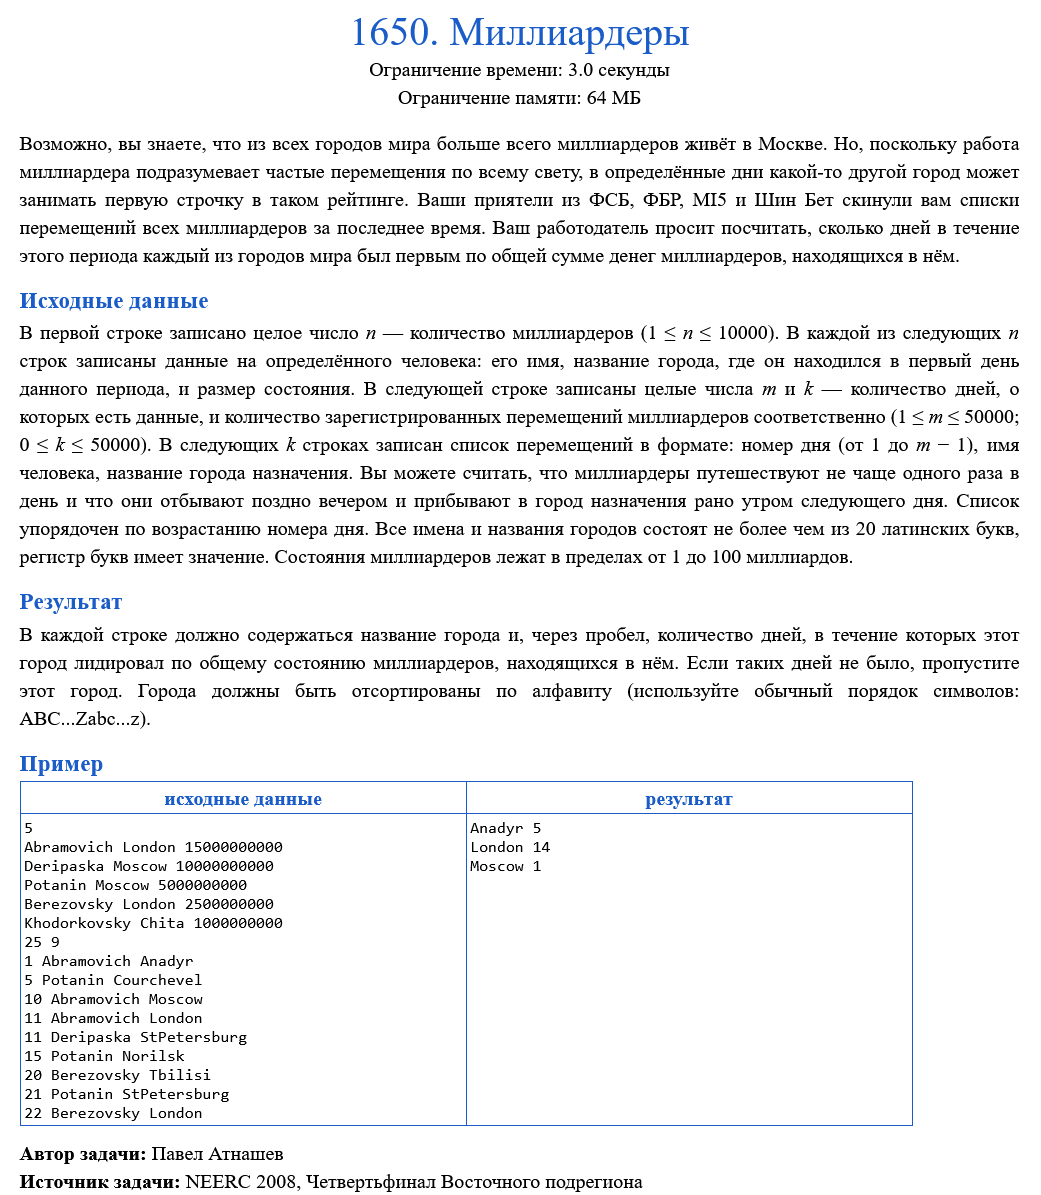
\includegraphics[width=0.9\linewidth]{pic/task_1650.png}}
\caption{Условие задачи 1650.}
\end{figure}

\subsection{Краткое описание алгоритма}
\textbf{1. Входные данные:} в первой строке записано целое число $n$ — количество миллиардеров $(1 \leq n \leq 10000)$. В каждой из следующих $n$ строк записаны данные на определённого человека: его имя, название города, где он находился в первый день данного периода, и размер состояния. \\

В следующей строке записаны целые числа $m$ и $k$ — количество дней, о которых есть данные, и количество зарегистрированных перемещений миллиардеров соответственно $(1 \leq m \leq 50000; 0 \leq k \leq 50000)$. В следующих $k$ строках записан список перемещений в формате: номер дня (от $1$ до $m - 1$), имя человека, название города назначения.\\

 Вы можете считать, что миллиардеры путешествуют не чаще одного раза в день и что они отбывают поздно вечером и прибывают в город назначения рано утром следующего дня. Список упорядочен по возрастанию номера дня. Все имена и названия городов состоят не более чем из 20 латинских букв, регистр букв имеет значение. Состояния миллиардеров лежат в пределах от 1 до 100 миллиардов \\

\textbf{2.}  Создадим структуру, в которой будут находиться отсортированные по неубыванию множество городов, в котором будем хранить актуальное состояние каждого из городов, в случае перелета миллиардера сумма города изменяется, соответственно заново сортируется структура;\\

\textbf{3.}  создадим еще одну структуру данных, в которой будем хранить имя миллиардера и информацию о городе, в котором он находится. Для этого будем использовать \textit{словарь} (или \textit{map}): ключ -- имя миллиардера, значение -- структура, в которой хранится информация о количестве денег и о длительности их нахождения в нем;\\

\textbf{4.} весь алгоритм работает за $O(n \cdot \ln n)$\\

\textbf{5. Выходные данные:} в каждой строке должно содержаться название города и, через пробел, количество дней, в течение которых этот город лидировал по общему состоянию миллиардеров, находящихся в нём. Если таких дней не было, пропустите этот город. Города должны быть отсортированы по алфавиту (используйте обычный порядок символов: ABC...Zabc...z). 

\subsection{Листинг}

\begin{center}
\begin{lstlisting}[label=some-code,caption={Исходный код для 1650}]
#include <iostream>
#include <map>
#include <set>


// structure for city parameters
struct City {
    std::string _name;
    long long _money;
    int _days;
} pCity[60000];

//structure for billionaires' parameters
struct Billionaire {
    long long _money;
    City *_loc;
} pBillionaire[10000];


int main() {

    int n, m, k;
    std::cin >> n;

    int _city_number = 0;

    std::map<std::string, City *> _cities;
    std::map<std::string, Billionaire *> _billionaires;
    std::set<std::pair<long long, City *>, std::greater<>> score;

    for (int i = 0; i < n; i++) {
        std::string name_person;
        std::string name_city;
        long long money;
        std::cin >> name_person >> name_city >> money;

        if (!_cities[name_city]) {

            pCity[_city_number]._name = name_city;
            pCity[_city_number]._money = money;
            _cities[name_city] = &pCity[_city_number++];

        } else _cities[name_city]->_money += money;


        pBillionaire[i]._money = money;
        pBillionaire[i]._loc = _cities[name_city];
        _billionaires[name_person] = &pBillionaire[i];

    }

    for (auto &item : _cities) {
        score.insert({item.second->_money, item.second});
    }

    int today = 0;

    std::cin >> m >> k;

    for (int i = 0; i < k; i++) {
        int day;
        std::string name_person;
        std::string name_city;
        std::cin >> day >> name_person >> name_city;

        int count = day - today;
        today = day;

        auto a = score.begin();
        auto b = a++;

        if (a->first < b->first || a == score.end()) {
            b->second->_days += count;
        }

        City *to_city = _cities[name_city];
        Billionaire *who = _billionaires[name_person];

        if (to_city == nullptr) {

            pCity[_city_number]._name = name_city;
            _cities[name_city] = &pCity[_city_number++];
            to_city = _cities[name_city];
        }

        score.erase({who->_loc->_money, who->_loc});
        score.erase({to_city->_money, to_city});

        who->_loc->_money -= who->_money;

        score.insert({who->_loc->_money, who->_loc});

        who->_loc = to_city;
        to_city->_money += who->_money;

        score.insert({to_city->_money, to_city});
    }

    int count = m - today;

    auto a = score.begin();
    auto b = a++;

    if (a->first < b->first || a == score.end()) {
        b->second->_days += count;
    }

    for (auto &item : _cities) {
        if (item.second->_days > 0) {
            std::cout << item.first << " " << item.second->_days << std::endl;
        }
    }

    return 0;
}
\end{lstlisting}
\end{center}

\newpage
\subsection{Результат}
\begin{figure}[h!]
\center{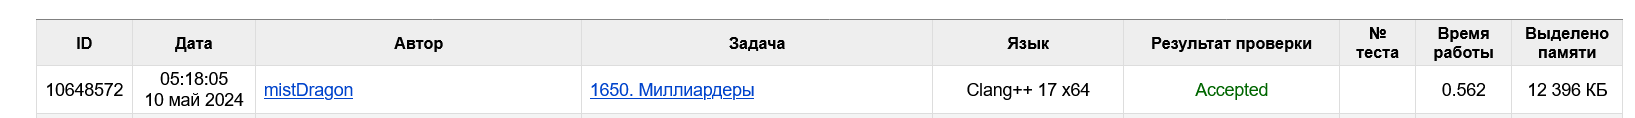
\includegraphics[width=1\linewidth]{pic/screen_1650.png}}
\caption{Результат отправки задачи 1650.}
\end{figure}







\newpage
\section{Задача 1450}

\begin{figure}[h!]
\center{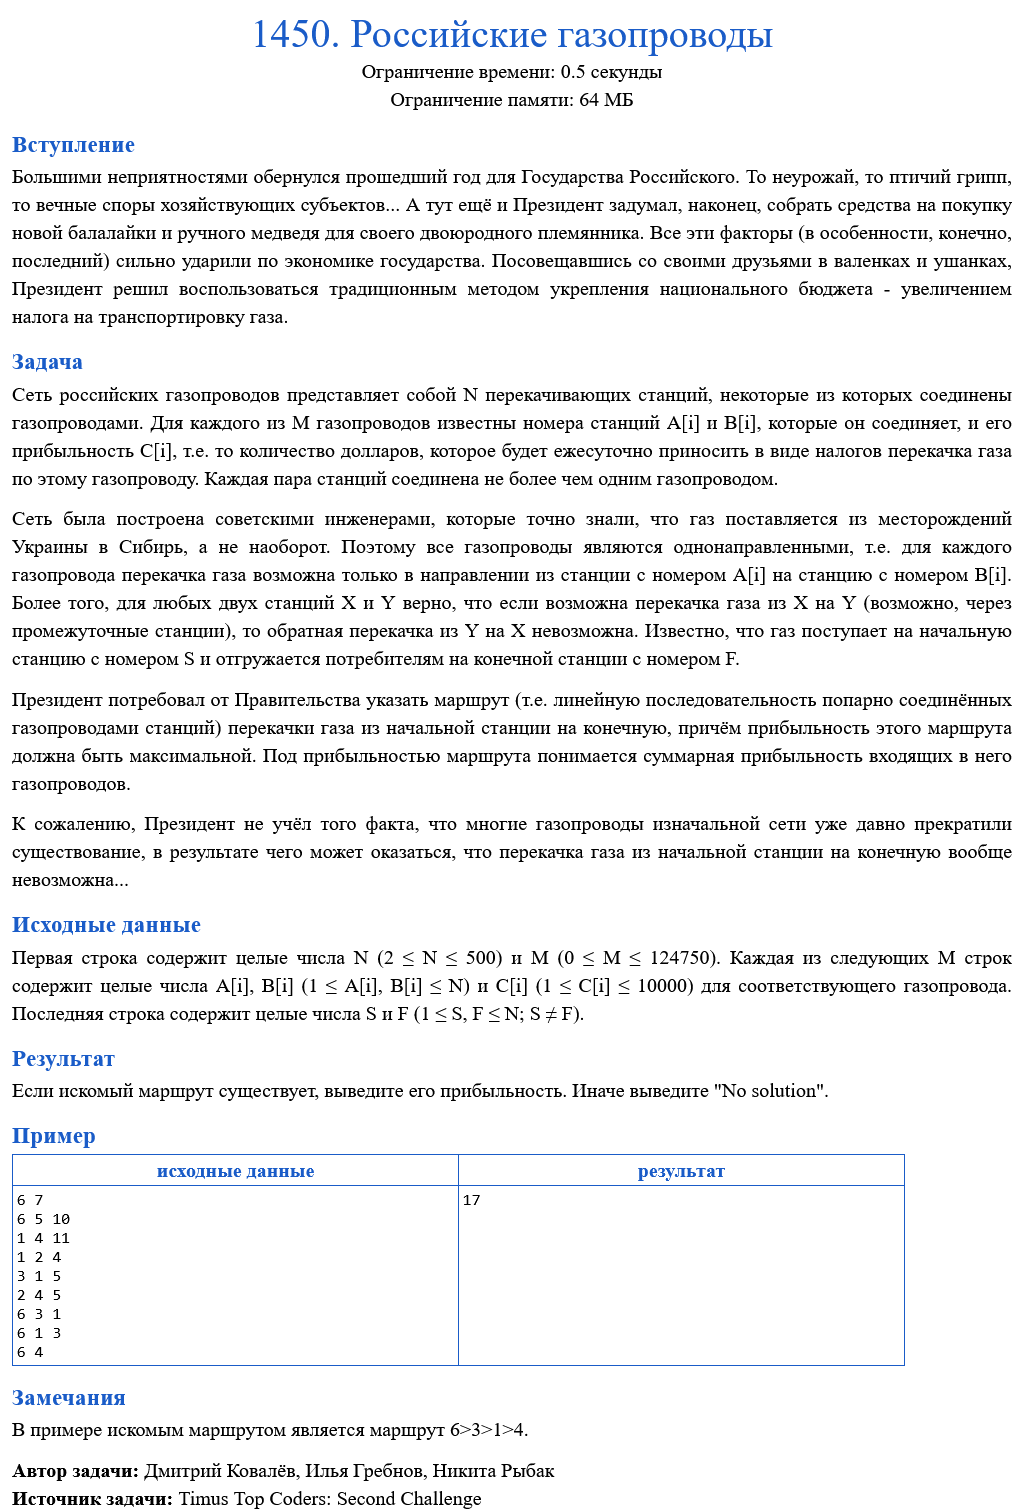
\includegraphics[width=0.8\linewidth]{pic/task_1450.png}}
\caption{Условие задачи 1450.}
\end{figure}

\subsection{Краткое описание алгоритма}
В основе решения лежит применение алгоритма \textbf{Форда-Беллмана} -- алгоритм нахождения кратчайшего пути из заданной вершины $s$ до всех остальных вершин взвешенного графа $G = \left( V, E \right)$. Если в графе $G$ есть циклю с отрицательным суммарным весом, притом достижимые из $s$, тогда кратчайших путей не существует.\\

\textbf{1. Входные данные:} первая строка содержит целые числа $N \, (2 \leq N \leq 500)$ и $M \, (0 \leq M \leq 124750)$. Каждая из следующих $M$ строк содержит целые числа $A[i], \, B[i] \, (1 \leq A[i],\, B[i] \leq N)$ и $C[i] \, (1 \leq C[i] \leq 10000)$ для соответствующего газопровода. Последняя строка содержит целые числа $S$ и $F \, (1 \leq S,\, F \leq N; S \neq F)$.\\

\textbf{2.} создадим отдельный массив, в котором будет фиксироваться максимальная газопроводность на каждом шаге; \\

\textbf{3.} на каждом шаге рассмотрим все пути из каждой посещенной вершины, в случае нахождения большего значения максимальной газопроводности в вершину $v$, обновляем значение по этому индексу в массиве из прошлого пункта; \\

\textbf{4.} таким образом, в массиве из пункта 2 будут находиться максимальные значения газопроводности, -1 означает, что такого пути нет.  \\

\textbf{5. Выходные данные:} если искомый маршрут существует, выведите его прибыльность. Иначе выведите "No solution".

\subsection{Листинг}

\begin{center}
\begin{lstlisting}[label=some-code,caption={Исходный код для 1450}]
#include <iostream>
#include <vector>


// structure to keep the edge
struct Way {
    int a, b, w;
};


int main() {

    std::ios_base::sync_with_stdio(0);
    std::cin.tie(0);
    std::cout.tie(0);

    int n, m, s, f;
    std::vector<Way> ways;
    std::vector<int> gas_transfer(500, -1);

    std::cin >> n >> m;

    for (int i = 0; i < m; ++i) {
        int a, b, w;
        std::cin >> a >> b >> w;
        ways.push_back({a - 1, b - 1, w});
    }

    std::cin >> s >> f;
    --s;
    --f;
    
    gas_transfer[s] = 0;

    for (int i = 0; i < n - 1; ++i) {
        for (int j = 0; j < m; ++j) {

            if (gas_transfer[ways[j].b] < gas_transfer[ways[j].a] + ways[j].w && gas_transfer[ways[j].a] != -1)
                gas_transfer[ways[j].b] = gas_transfer[ways[j].a] + ways[j].w;
        }
    }

    if (gas_transfer[f] != -1) std::cout << gas_transfer[f];
    else std::cout << "No solution";

    return 0;
}
\end{lstlisting}
\end{center}

\subsection{Результат}
\begin{figure}[h!]
\center{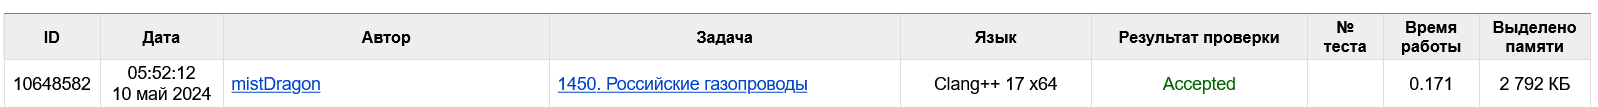
\includegraphics[width=0.9\linewidth]{pic/screen_1450.png}}
\caption{Результат отправки задачи 1450.}
\end{figure}









\newpage

\section{Задача 1806}

\begin{figure}[h!]
\center{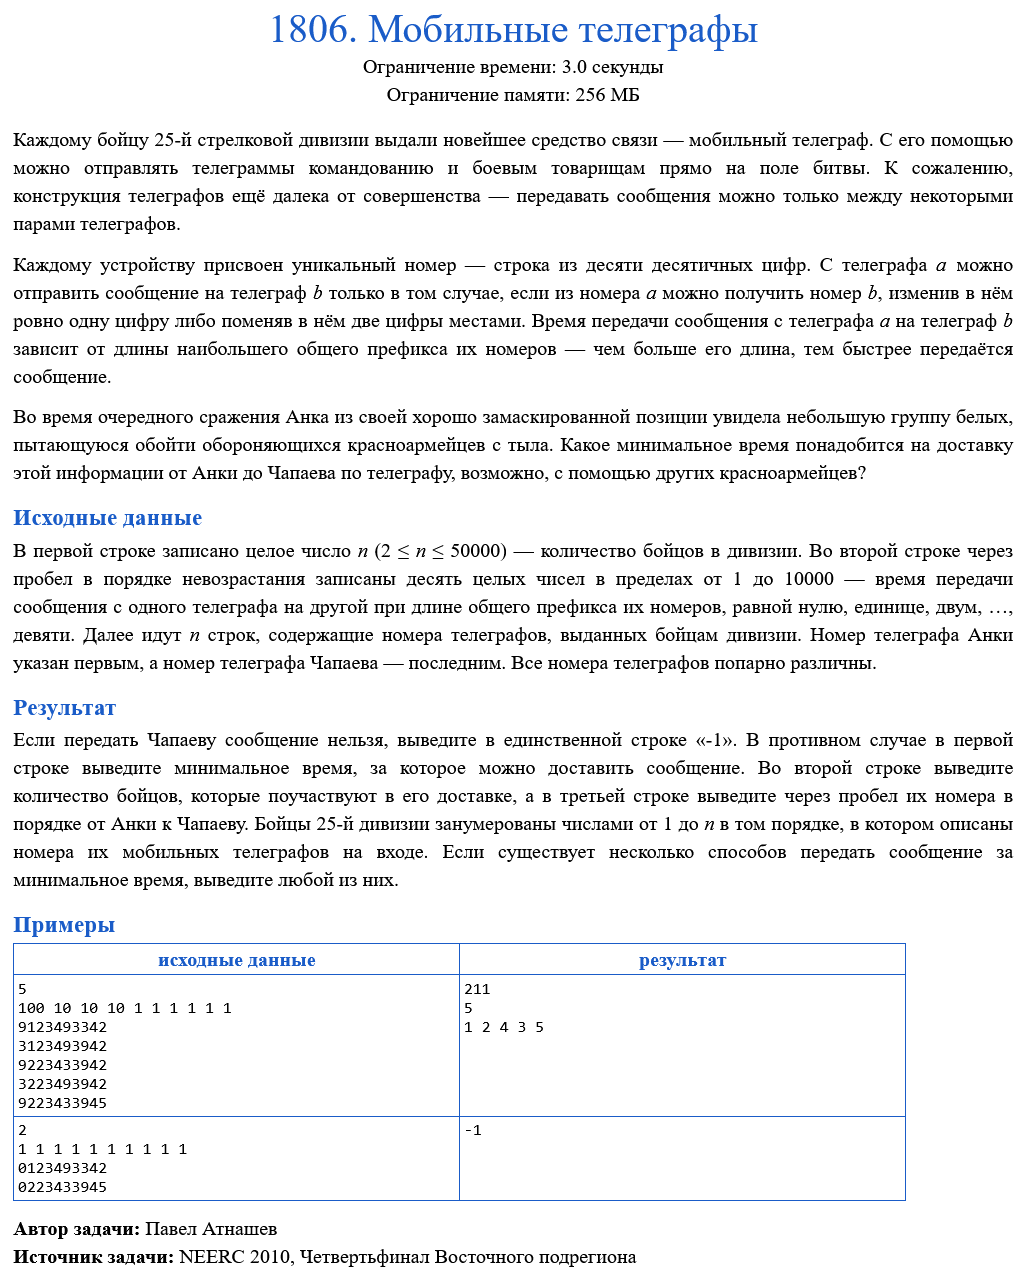
\includegraphics[width=0.9\linewidth]{pic/task_1806.png}}
\caption{Условие задачи 1806.}
\end{figure}

\subsection{Краткое описание алгоритма}
В основе решения задачи лежит \textbf{алгоритм Дейкстры} -- алгоритм находждения кратчайших путей от одной из вершин графа до всех остальных.\\

Каждой вершине из множества вершин V сопоставим метку — минимальное известное расстояние от этой вершины до стартовой вершины a.
Алгоритм работает пошагово — на каждом шаге он «посещает» одну вершину и пытается уменьшать метки. Метка самой вершины a полагается равной 0, метки остальных вершин — бесконечности. Это отражает то, что расстояния от a до других вершин пока неизвестны. Все вершины графа помечаются как непосещённые.\\

 Если все вершины посещены, алгоритм завершается. В противном случае, из ещё не посещённых вершин выбирается вершина u, имеющая минимальную метку. Мы рассматриваем всевозможные маршруты, в которых u является предпоследним пунктом. Вершины, в которые ведут рёбра из u, назовём соседями этой вершины. Для каждого соседа вершины u, кроме отмеченных как посещённые, рассмотрим новую длину пути, равную сумме значений текущей метки u и длины ребра, соединяющего u с этим соседом. Если полученное значение длины меньше значения метки соседа, заменим значение метки полученным значением длины. Работа алгоритма завершается, когда все вершины посещены. \\


\textbf{1. Входные данные:} в первой строке записано целое число $n$ $(2 \leq n \leq 50000)$ — количество бойцов в дивизии. Во второй строке через пробел в порядке невозрастания записаны десять целых чисел в пределах от $1$ до $10000$ — время передачи сообщения с одного телеграфа на другой при длине общего префикса их номеров, равной нулю, единице, двум, …, девяти. Далее идут $n$ строк, содержащие номера телеграфов, выданных бойцам дивизии. Номер телеграфа Анки указан первым, а номер телеграфа Чапаева — последним. Все номера телеграфов попарно различны.  \\

\textbf{2.}  Строим граф;\\

\textbf{3.} Находим кратчайшее расстояние, с помощью алгоритма Дейкстры \\

\textbf{4. Выходные данные:} если передать Чапаеву сообщение нельзя, выведите в единственной строке «-1». В противном случае в первой строке выведите минимальное время, за которое можно доставить сообщение. Во второй строке выведите количество бойцов, которые поучаствуют в его доставке, а в третьей строке выведите через пробел их номера в порядке от Анки к Чапаеву. Бойцы $25$-й дивизии занумерованы числами от $1$ до $n$ в том порядке, в котором описаны номера их мобильных телеграфов на входе. Если существует несколько способов передать сообщение за минимальное время, выведите любой из них.

\subsection{Листинг}

\begin{center}
\begin{lstlisting}[label=some-code,caption={Исходный код для 1806}]
#include <iostream>
#include <vector>
#include <unordered_map>
#include <queue>


const int inf = 1e9 + 7;
const int width = 10;
const int max_n = 50000;

long long pw[width]; // 1, 10, 100 ...
int cost[width]; // The costs of the prefix matching

struct Node {
    std::vector<std::pair<int, Node*>> v; // Neighbors <cost, Node*>
    Node* parent{}; // Of the shortest path
    int d{}; // Shortest path cost
    bool visited{};
} nodes[max_n];

std::unordered_map<long long, Node*> m;

int getDigit(long long num, int i) {
    return (int) (num / pw[i] % 10);
}

long long setDigit(long long num, int i, int d) {
    return num - ((long long) getDigit(num, i)) * pw[i] + d * pw[i];
}

int matchPrefix(long long num1, long long num2) {
    int matched = 0;

    for (int i = width - 1; i >= 0; i--) {
        if (getDigit(num1, i) == getDigit(num2, i)) {
            matched++;
        } else {
            break;
        }
    }

    return matched;
}

// Adds this station into the graph at node #id
void add(long long num, int id) {
    std::vector<std::pair<int, Node*>> v;

    // Replace digit
    for (int i = 0; i < width; i++) {
        for (int d = 0; d < 10; d++) {
            auto num2 = setDigit(num, i, d);

            if (m.find(num2) != m.end()) {
                int c = cost[matchPrefix(num, num2)];
                v.emplace_back( c, (*m.find(num2)).second );
            }
        }
    }

    // Switch two digits
    for (int i = 0; i < width; i++) {
        for (int j = i + 1; j < width; j++) {
            int di = getDigit(num, i);
            int dj = getDigit(num, j);

            auto num2 = setDigit(setDigit(num, j, di), i, dj);

            if(m.find(num2) != m.end()) {
                int c = cost[matchPrefix(num, num2)];
                v.emplace_back( c, (*m.find(num2)).second );
            }
        }
    }

    m[num] = &nodes[id];

    for(auto p : v){
        p.second->v.emplace_back( p.first, &nodes[id] );
        nodes[id].v.emplace_back( p.first, p.second );
    }
}

//  Dijkstras algorithm
void dijkstra(Node* start, int n) {

    using pin = std::pair<int, Node*>;
    std::priority_queue<pin, std::vector<pin>, std::greater<>> q;

    for (int i = 0; i < n; ++i) nodes[i].d = inf, nodes[i].visited = false;

    start->d = 0;

    q.push( { 0, start } );

    while(!q.empty()) {

        auto p = q.top();
        q.pop();
        auto node = p.second;

        if (node->visited) continue;

        node->visited = true;

        for (auto it = node->v.begin(); it < node->v.end(); it++) {
            auto u = (*it).second;
            int cur_cost = (*it).first;

            if (!u->visited && u->d > node->d + cur_cost) {
                u->parent = node;
                u->d = node->d + cur_cost;
                q.push( { u->d, u });
            }
        }
    }
}

int main() {

    int n;
    std::cin >> n;

    long long b = 1;

    for (long long & i : pw) i = b, b *= 10;

    for (int & i : cost) std::cin >> i;

    for (int i = 0; i < n; i++) {
        long long num;
        std::cin >> num;
        add(num, i);
    }

    std::vector<Node*> result;
    dijkstra(&nodes[0], n);

    if (!nodes[n - 1].visited) {
        std::cout << -1;
        return 0;
    }

    std::cout << nodes[n - 1].d << "\n";

    for (Node* node = &nodes[n - 1]; node; node = node->parent) result.push_back(node);

    std::cout << result.size() << "\n";

    for (auto item = result.rbegin(); item < result.rend(); ++item)
        std::cout << 1 + (*item-nodes) << " ";
}

\end{lstlisting}
\end{center}

\subsection{Результат}
\begin{figure}[h!]
\center{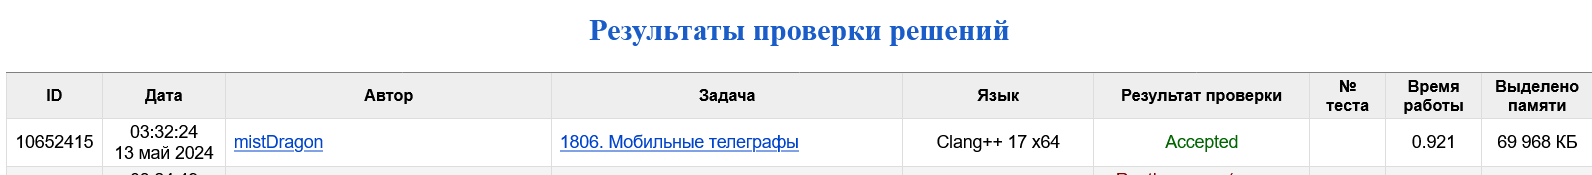
\includegraphics[width=0.9\linewidth]{pic/screen_1806.png}}
\caption{Результат отправки задачи 1806.}
\end{figure}



\newpage
\section{Вывод по работе}
В ходе выполнения данной лабораторной работы были реализованы алгоритмы для решения задач $1650$, $1450$ и $1806$.\\

 В задаче  $1450$ был применен алгоритм \textbf{Форда-Беллмана}, в $1806$ -- \textbf{алгоритм Дейкстры}.
\end{document}













